\documentclass[10pt,twocolumn,letterpaper]{article}

\usepackage{cvpr}
\usepackage{times}
\usepackage{epsfig}
\usepackage{graphicx}
\usepackage{amsmath}
\usepackage[section]{placeins}
\usepackage{amssymb}
\usepackage{float}
\usepackage[ruled,linesnumbered]{algorithm2e}
\usepackage{longtable}
\usepackage{booktabs}
\usepackage{array}
\usepackage{caption}
\usepackage{subcaption}

\graphicspath{ {./graphs/} }

% Include other packages here, before hyperref.

% If you comment hyperref and then uncomment it, you should delete
% egpaper.aux before re-running latex.  (Or just hit 'q' on the first latex
% run, let it finish, and you should be clear).
\usepackage[colorlinks=true, citecolor=blue]{hyperref}


\cvprfinalcopy % *** Uncomment this line for the final submission

\def\cvprPaperID{****} % *** Enter the CVPR Paper ID here
\def\httilde{\mbox{\tt\raisebox{-.5ex}{\symbol{126}}}}

% Pages are numbered in submission mode, and unnumbered in camera-ready
%\ifcvprfinal\pagestyle{empty}\fi
\setcounter{page}{1}
\begin{document}

%%%%%%%%% TITLE
\title{A Training Method For \textit{VideoPose3D} with Action Recognition}

\author{Hao Bai\\
Zhejiang University - University of Illinois at Urbana-Champaign Institute, ZJUI\\
Haining, Jiaxing\\
{\tt\small https://jackgetup.com, Haob.19@intl.zju.edu.cn}
% For a paper whose authors are all at the same institution,
% omit the following lines up until the closing ``}''.
% Additional authors and addresses can be added with ``\and'',
% just like the second author.
% To save space, use either the email address or home page, not both
%\and
%\textbf{Prof.} Gaoang Wang\\
%ZJU-UIUC Institute\\
%Haining, Jiaxing\\
%{\tt\small gaoangwang@intl.zju.edu.cn}
}

\maketitle
%\thispagestyle{empty}

%%%%%%%%% ABSTRACT
\begin{abstract}
	Action recognition and pose estimation from video are closely related tasks for understanding
	human motions, but the work to utilize both is rare in literature. In this essay I show an 
	action-recognition-based training method for \textit{VideoPose3D}, which contributes to the 
	precision of velocity error and speed of training. The model is fed with videos which have exactly 
	the same type of action in the estimation period, and it only requires a small amount of data. 
	Evidence has shown that under a limited amount of epochs and data, our approach outperforms 
	the original research. The code of this project, is available under the open-source MIT License at
	\url{https://github.com/BiEchi/Pose3dDirectionalTraining}. 
   

\end{abstract}

%%%%%%%%% BODY TEXT
\section{Introduction}

Vision-based human motion analysis attempts to understand the movements of the human body 
using computer vision and machine learning techniques. Technically speaking, the main goal
for pose estimation and motion analysis is to rebuild the movements of the locations for 
human body joints inside videos. Qualitative speaking, lower estimation error means better 
performance.


The effect between pose estimation and action recognition is mutual. Pose estimation
and action recognition can utilize the same dataset \cite{jhuang2013towards, andriluka2018posetrack}
Pose estimation can be used for action recognition, with the conclusion that a lower
estimation error leads to a more accurate classification of action recognition \cite{yao2011does}. 
Turning around, action priors and also be used to ameliorate the precision of pose estimation 
\cite{yao2012coupled, iqbal2017pose, gall20102d}. There have also been work combining these two tasks 
together and perform better in each field \cite{7298734, luvizon20182d}.


In the field of 3D post estimation by deep learning approach, there are many successful creatures 
with various types of training methods, like Maximum-Margin Structured training by Li et al. 
\cite{li2015maximum}, Feedback Loop training by Oberweger et al.\cite{oberweger2015training}, and 
also Semi-Supervised training by Pavllo et al. \cite{pavllo20193d}, which we mainly concern with 
in our work.

\textit{VideoPose3D} has been very successful because of its high performance and SOTA precision.
This work utilizes the datasets \textbf{HumanEva} \cite{sigal2010humaneva} and \textbf{Human3.6M} 
\cite{ionescu2013human3}. \textbf{Human3.6M} has 11 subjects and 4 viewpoints in total, and 15 types of actions.
We've got our motivation that, \textit{VideoPose3D} takes a variety of (instead of a certain type of) actions 
as training data, but there have been lots of successful cases when using action recognition for pose estimations 
works well for improving its performance, which gives rise to our project.

%------------------------------------------------------------------------
\section{Related Works and Our Contributions}

As mentioned in the Introduction part, our work is based on the previous work \textit{VideoPose3D} 
\cite{pavllo20193d} and gets its motivation from successful cases to utilize action recognition for 
pose estimation \cite{yao2012coupled, iqbal2017pose, gall20102d}. In this part we illustrate how
these works model and how we can utilize them to perform a better work based on them.

%-------------------------------------------------------------------------
\subsection{VideoPose3D}

\textit{VideoPose3D} was the state-of-the-art approach which "utilizes a fully convolutional model based on dilated 
temporal convolutions over 2D keypoints" \cite{pavllo20193d}. In early researches the main solution was to use recurrent 
neural networks (RNN) \cite{lee2018propagating}, but the research \textit{VideoPose3D} utilized the convolutional 
neuron network (CNN) to gain an efficient result on the dataset \textit{Human3.6M}, with the inspiration that
many authors had mentioned CNN in temporal models.

Technically speaking, \textit{VideoPose3D} takes a series of images as the input of the training network to imitate the
functionality as RNN (Figure \ref{CNN_in_VideoPose3D}). This ideology has been widely accepted in the current academy and there have been lots of successful
cases utilizing this method, e.g. the Spatial-Temporal-CNN used for crowd counting in videos \cite{miao2019st}, and LSTM-CNN
used for face anti-spoofing \cite{xu2015learning}. From these researches we see the capability of CNN. However, CNN is not a natural temporal
network itself, which means it bears a trait of parallelism and lack of temporal memory \cite{shin2016deep}.

\begin{figure}[H]
	\begin{center}
		%\fbox{\rule{0pt}{2in} \rule{0.9\linewidth}{0pt}}
  		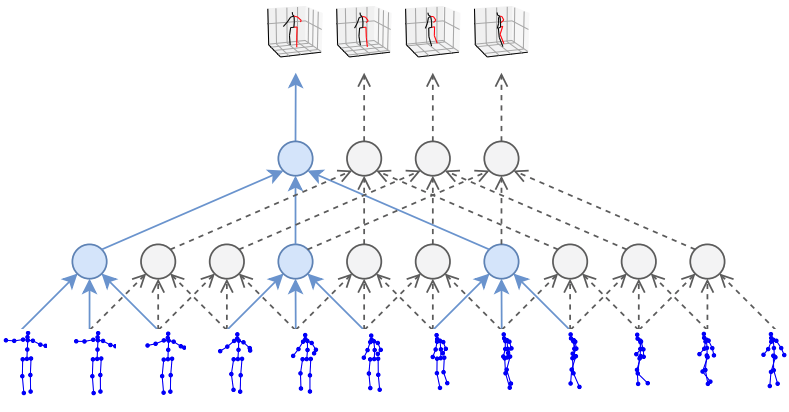
\includegraphics[width=1.0\linewidth]{CNN_in_VideoPose3D.png}
	\end{center}
   	\caption{The temporal convilutional model from \textit{VideoPose3D} takes 2D keypoint sequences (bottom) as input and 
   			 generates 3D pose estimation as out (top).}
	\label{CNN_in_VideoPose3D}
\end{figure}


The overall model of \textit{VideoPose3D} is a semi-supervised learning method (Figure 1). 

\begin{figure}[H]
	\begin{center}
		%\fbox{\rule{0pt}{2in} \rule{0.9\linewidth}{0pt}}
  		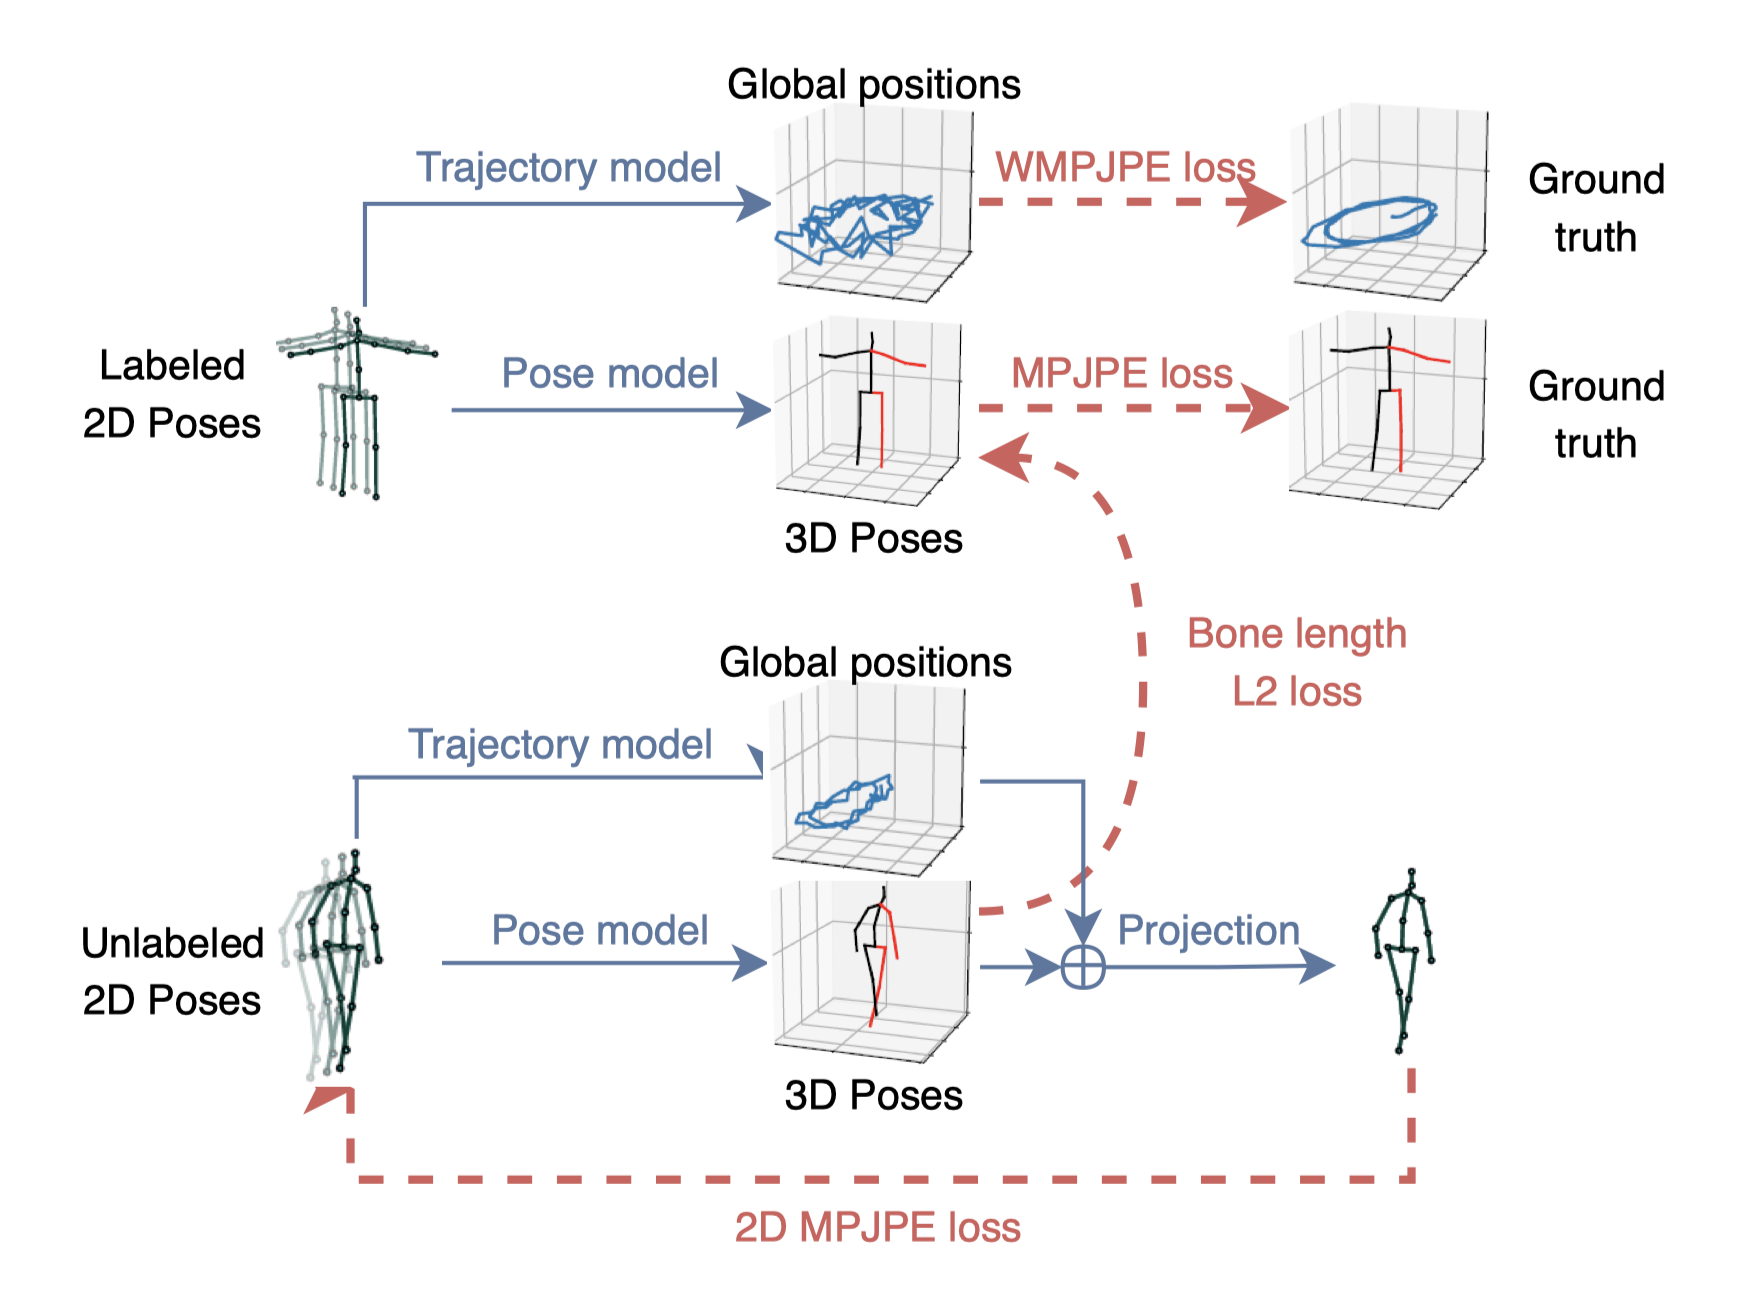
\includegraphics[width=0.9\linewidth]{original.png}
	\end{center}
   	\caption{The overall model of \textit{VideoPose3D}}
	\label{fig:long}
	\label{fig:onecol}
\end{figure}

%-------------------------------------------------------------------------
\subsection{Action Recognition}

The idea of homogenized learning was proposed firstly by Action Estimations \cite{wang2013action}. 
Hitherto, there have been a variety of researches focusing on the combination of action recognition and pose
estimation \cite{yao2012coupled}. The basic idea is to begin with 2D appearance-based action recognition
based on low-level appearance features. Outputs of the 2D action recognition are used as a prior distribution
for the particle-based optimization for 3D pose estimation. Finally, 3D pose-based action recognition is then 
performed based on pose features extracted from the estimated poses.

\begin{figure}[H]
	\begin{center}
		%\fbox{\rule{0pt}{2in} \rule{0.9\linewidth}{0pt}}
  		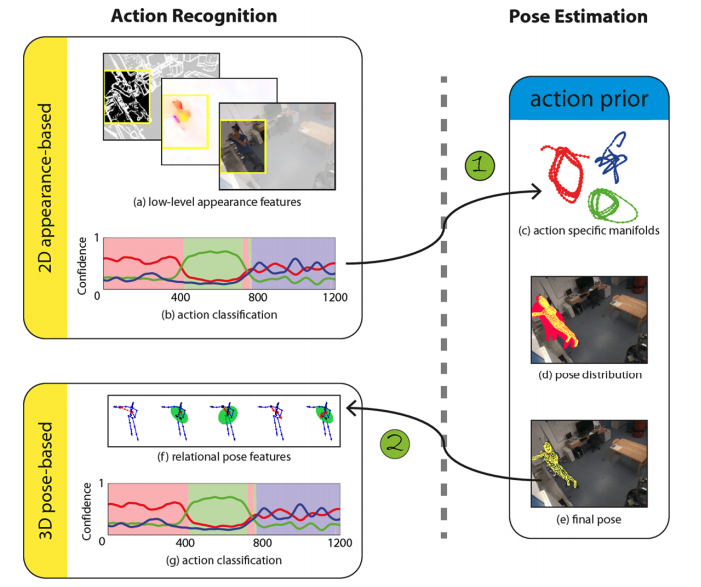
\includegraphics[width=0.9\linewidth]{action_and_pose.png}
	\end{center}
   	\caption{The coupled action recognition and pose estimation framework forwarded by \cite{yao2012coupled}.}
	\label{fig:long}
	\label{fig:onecol}
\end{figure}


%-------------------------------------------------------------------------
\subsection{Homography Estimation}

The idea of using homonegeious actions in a dataset was also inspired from Homography Estimation
in some deep images \cite{detone2016deep}.



%------------------------------------------------------------------------
\section{Representation and Modeling}
 
The detailed experimental setup can also be explored in \textit{README.md} in the github repo. To reproduce
the results, you need to test for 15 times for each type of action, and it's preferable to test for multiple
times. It's more convenient to use \textit{bash} scripts to save time.


Our work focuses on using certain types of actions for training data. For example, say there are 4 actions for all
subjects, i.e. sitting, walking, discussing, and posing. The original \textit{VideoPose3D} model takes all 4 types
of data as training data (Figure \ref{fig:model_comparison}, left), and they estimate results for all action in the end. Our model, instead, takes 
only one action as training data (Figure \ref{fig:model_comparison}, right), and we estimate ONLY result for this certain action in the end. Absolutely, this
process will iterate through all actions if all of them need to be estimated.

\begin{figure*}
\centering
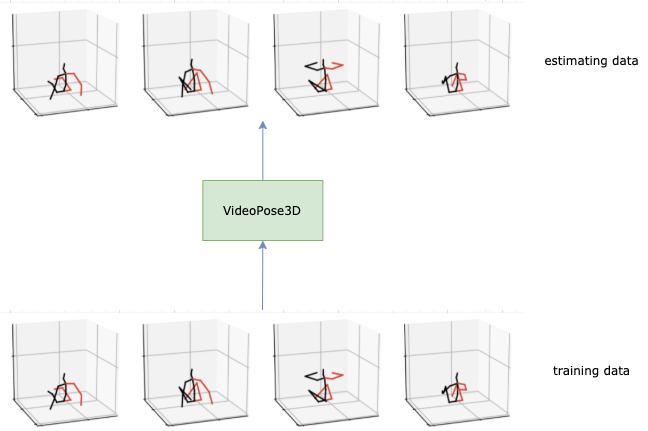
\includegraphics[width=8cm]{model.png}
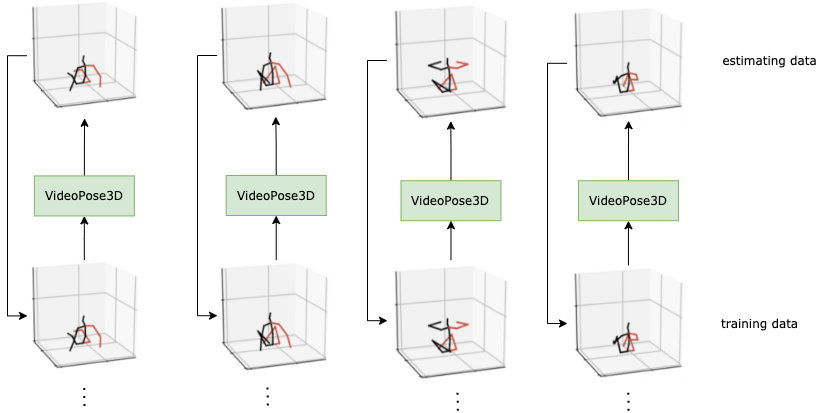
\includegraphics[width=8cm]{new_model.png}
\caption{The comparison of the original model (left) and our model (right). The original model takes all types of actions for 
		 training, but we only take a certain type of data as training data, as an approach to utilize action recognition for pose estimation.}
\label{fig:model_comparison}
\end{figure*}

Compared to the original model we utilized a different data-processing approach. The original approach
mentioned in \textit{VideoPose3D} uses all actions in training data, and the estimating effect was good
overall. We utilize the method that we only take one type of action for training, and the total amount 
for training should be the same. Mathematically, take the action \textit{Sitting} for example, it can 
be expressed as*

\begin{equation}
	\sum_{i\in actions}{f(i)} = f(Sitting)\cdot t
\end{equation}

where $f$ stands for the frames of subject, and $t$ means the number of epochs of our action-based 
training. Note that the unit of $t$ is unit-epoch instead of epoch. The unit-epoch stands for 1 epoch
of one action. According to the dataset we utilize, \textit{Human3.6M}, there are 15 actions for each
subject. Thus, the relationship between epoch and unit-epoch can be expressed mathematically as below.

\begin{equation}
	t_0 = t_{unit}\cdot 15
\end{equation}


In this approach, we utilize only one time of action, which means we save more data; and we also produce
the results in the same time, the evidence can be illustrated by formula (1). After testing, we conclude 
that our work outperforms the original work by 11\%.

The principle of our work is shown below.

In our model we also changed the process of training in the original research. In the original research,
it takes 15 unit-epochs to run a single epoch, because there are 15 types of actions. In our work, we can
tweak the number of unit-epochs not necessarily to be a multiple of 15, which makes it more flexible to 
observe and iterate. Shown below is the algorithm for our iterative training when not so many epochs are 
available (we take 2 epochs for example).


\begin{algorithm}
  \caption{Original \textit{VideoPose3D} Model}
  \SetAlgoLined
  
  \KwData{Training data, testing data, ground-truth data, total training epoch = 2.}
  \KwResult{Error value.}
  
  \For{\textsc{epoch} in \textsc{2}}
  	{
 		\textsc{Err}=VideoPose3D(\textsc{Train, Test, GT})\;
  		print(\textsc{Err})\;
  		
  	}
  
 \Return{\textsc{Err}}\;
\end{algorithm}

\begin{algorithm}
  \caption{Our Action-based Approach}
  \SetAlgoLined
  
  \KwData{Training data, testing data, ground-truth data, total training epoch = 2, action type.}
  \KwResult{Error value.}
  
  \For{\textsc{epoch} in $2\cdot 15$}
  	{
 		\textsc{Err for Action}=\textbf{VideoPose3D}(\textsc{Train, Test, GT, Action})\;
  		\textbf{print}(\textsc{Err for Action})\;
  		
  	}
  
 \Return{\textsc{Err for Action}}\;
\end{algorithm}



%------------------------------------------------------------------------

\section{Experiments}

Shown below are the results of the experiment. Expect a minor error when testing on your own. Note that all
unit are millimeter.

\subsection{Argument-based Training Results}

In this part we estimate the errors with different combinations of arguments for model training. The epoch of the original test was set to 
be 15 unit epochs (i.e. 1 epoch), and the epoch of the action-based test was set to 1 epoch. In the table below (Table \ref{tab:MPJPE Error} \&
Table \ref{tab:V-MPJPE Error}), we illustrate the pose estimation results with respect to different types of model with different
training arguments (i.e. the number of receptive field Frames \textbf{F}, the number of Unit Epochs \textbf{UE}),
15 different actions, and two different protocols (i.e. MPJPE and Velocity Error of MPJPE).

In the tables the model with the best performance is in bold, and we set the argument as the highest classification standard
for better comparison. The visualized Argument part is labeled in the corresponding letter of Figure \ref{fig:four_error_graphs}.


\begin{center}
\begin{table*}
\small
%\begin{tabular}{cl | p{0.4cm} p{0.4cm} p{0.3cm} p{0.5cm}p{0.6cm}p{0.5cm}p{0.3cm}p{0.4cm}p{0.1cm}p{0.4cm}p{0.7cm}p{0.4cm}p{0.8cm}p{0.4cm}p{0.8cm} p{0.3cm} } 
\setlength\tabcolsep{2.3pt}
\begin{tabular}{l|l|rrrrrrrrrrrrrrrr}
Arguments & Model & Dir. & Disc. & Eat & Greet & Phone & Photo & Pose & Purch. & Sit & SitD. & Smoke & Wait & WkD. & Walk & WkT. & \textbf{Avg} \\

\hline
1F, 15 UE (a) & VideoPose3D & 67.0 & \textbf{65.8} & 68.7 & 72.5 & \textbf{74.2} & \textbf{87.2} & \textbf{65.5} & \textbf{73.1} & 85.6 & 117 & 73.6 & \textbf{70.8} & 81.1 & 63.5 & 67.3 & 75.5 \\
1F, 15 UE & Ours & \textbf{61.9} & 69.2 & \textbf{62.0} & \textbf{68.4} & 75.7 & 88.2 & 74.5 & 76.9 & \textbf{81.5} & \textbf{97.9} & \textbf{71.1} & 80.9 & \textbf{80.7} & \textbf{49.9} & \textbf{59.2} & \textbf{73.2}\\

\hline


27F, 15 UE (b) & VideoPose3D & \textbf{54.5} & \textbf{61.4} & 56.3 & \textbf{58.6} & \textbf{61.3} & \textbf{68.6} & \textbf{57.6} & \textbf{60.6} & 70.5 & 84.7 & 60.5 & \textbf{59.1} & 68.2 & 51.8 & \textbf{53.1} & \textbf{61.8} \\
27F, 15 UE & Ours & 70.5 & 71.9 & \textbf{52.1} & 61.4 & 69.0 & 82.6 & 70.6 & 82.1 & \textbf{70.4} & \textbf{79.4} & \textbf{60.3} & 79.5 & \textbf{56.1} & \textbf{44.2} & 56.2 & 67.1\\
\hline

243F, 1200 UE & Pavlakos \cite{pavlakos2017coarse} & 67.4 & 71.9 & 66.7 & 69.1 & 72.0 & 77.0 & 65.0 & 68.3 & 83.7 & 96.5 & 71.7 & 65.8 & 74.9 & 59.1 & 63.2 & 71.9 \\
243F, 1200 UE & Luvizon \cite{luvizon20182d} & 49.2 & 51.6 & 47.6 & 50.5 & 51.8 & 60.3 & 48.5 & 51.7 & 61.5 & 70.9 & 53.7 & 48.9 & 57.9 & 44.4 & 48.9 & 53.2\\
243F, 1200 UE & VideoPose3D & \textbf{46.6} & \textbf{47.4} & 45.2 & \textbf{46.2} & \textbf{49.0} & \textbf{56.7} & \textbf{46.4} & \textbf{47.2} & \textbf{59.9} & 68.2 & \textbf{48.1} & \textbf{46.2} & 49.4 & 32.9 & \textbf{34.3} & \textbf{48.2}\\
243F, 1200 UE & Ours & 47.9 & 48.8 & \textbf{45.1} & 48.4 & 51.7 & 62.8 & 47.1 & 59.4 & 61.2 & \textbf{64.7} & 48.2 & 59.3 & \textbf{46.6} & \textbf{31.4} & 35.5 & 50.5\\
 
\hline 

\hline
\end{tabular}

\caption{Protocol 1, MPJPE Error}
\label{tab:MPJPE Error}
\end{table*}
\end{center}


\begin{center}
\begin{table*}
\small
%\begin{tabular}{l | p{0.4cm} p{0.4cm} p{0.3cm} p{0.5cm}p{0.6cm}p{0.5cm}p{0.3cm}p{0.4cm}p{0.1cm}p{0.4cm}p{0.7cm}p{0.4cm}p{0.8cm}p{0.4cm}p{0.8cm} p{0.3cm} } 
\setlength\tabcolsep{2.3pt}
\begin{tabular}{l|l|rrrrrrrrrrrrrrrr} 
Arguments & Model & Dir. & Disc. & Eat & Greet & Phone & Photo & Pose & Purch. & Sit & SitD. & Smoke & Wait & WkD. & Walk & WkT. & \textbf{Avg} \\
\hline
1F, 15 UE (c) & VideoPose3D & \textbf{10.7} & \textbf{12.2} & 10.2 & 12.4 & 11.1 & \textbf{11.0} & 10.5 & 12.3 & \textbf{11.4} & \textbf{13.8} & 11.0 & \textbf{10.6} & 12.7 & 12.9 & 12.4 & 11.7  \\
1F, 15 UE & Ours & 10.9 & 13.0 & \textbf{9.59} & \textbf{11.8} & \textbf{10.3} & 11.4 & \textbf{10.1} & \textbf{10.5} & 12.2 & 14.6 & \textbf{10.9} & 11.5 & \textbf{12.5} & \textbf{12.6} & \textbf{12.2} & \textbf{11.6} \\
\hline
27F, 15 UE (d) & VideoPose3D & 3.84 & 4.02 & 3.14 & 4.42 & 3.31 & 3.58 & \textbf{3.44} & 3.93 & 3.14 & 4.21 & 3.36 & \textbf{3.34} & 4.68 & 4.51 & 4.08 & 3.80 \\
27F, 15 UE & Ours & \textbf{3.78} & \textbf{4.28} & \textbf{3.01} & \textbf{4.27} & \textbf{3.14} & \textbf{3.50} & 3.79 & \textbf{3.65} & \textbf{2.84} & \textbf{3.90} & \textbf{3.05} & 3.55 & \textbf{4.37} & \textbf{3.77} & \textbf{3.49} & \textbf{3.63}\\
\hline

243F, 1200 UE & VideoPose3D & \textbf{3.01} & 3.21 & \textbf{2.33} & \textbf{3.55} & 2.33 & \textbf{2.83} & \textbf{2.77} & 3.23 & 2.11 & 3.01 & 2.44 & \textbf{2.43} & 3.82 & 3.33 & \textbf{2.86} & \textbf{2.49} \\
243F, 1200 UE & Ours & 3.14 & \textbf{3.20} & 2.48 & 3.62 & \textbf{2.31} & 2.91 & 3.04 & \textbf{3.11} & \textbf{2.07} & \textbf{2.88} & \textbf{2.23} & 2.73 & \textbf{3.66} & \textbf{3.04} & 2.97 & 3.08 \\

 
\hline

\hline
\end{tabular}

\caption{Protocol 2, MPJPE Velocity Error}
\label{tab:V-MPJPE Error}
\end{table*}
\end{center}

\begin{figure*}
     \centering
     \begin{subfigure}[b]{0.49\textwidth}
         \centering
         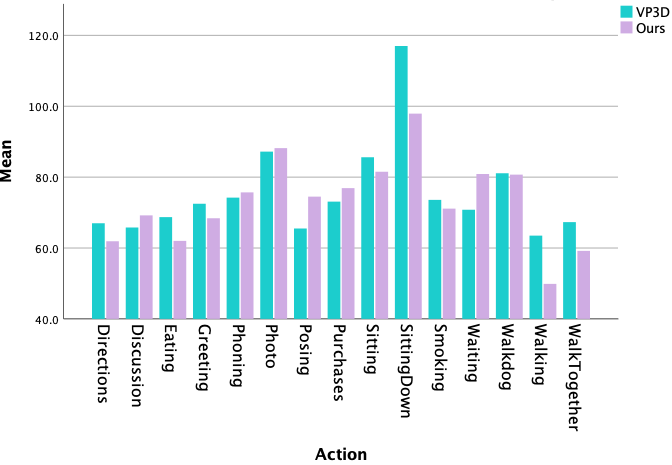
\includegraphics[width=\textwidth]{mean_error_comparison.png}
         \caption{1F, 15UE, MPJPE}
         \label{fig:est_a}
     \end{subfigure}
     \hfill
     \begin{subfigure}[b]{0.49\textwidth}
         \centering
         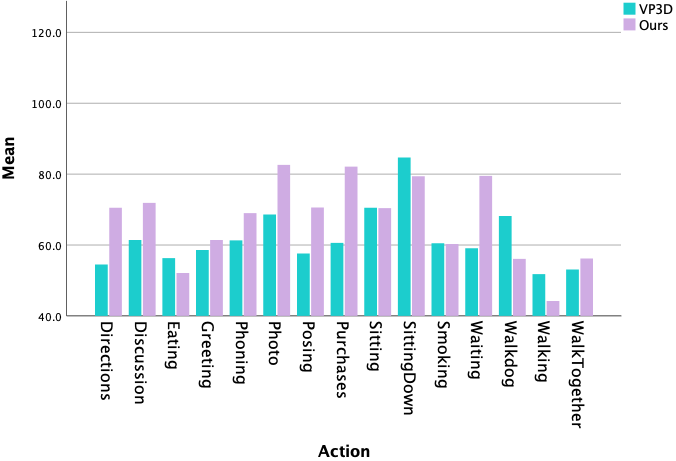
\includegraphics[width=\textwidth]{mean_error_comparison_2.png}
         \caption{27F, 15UE, MPJPE}
         \label{fig:est_b}
     \end{subfigure}
     \quad
     \begin{subfigure}[b]{0.49\textwidth}
         \centering
         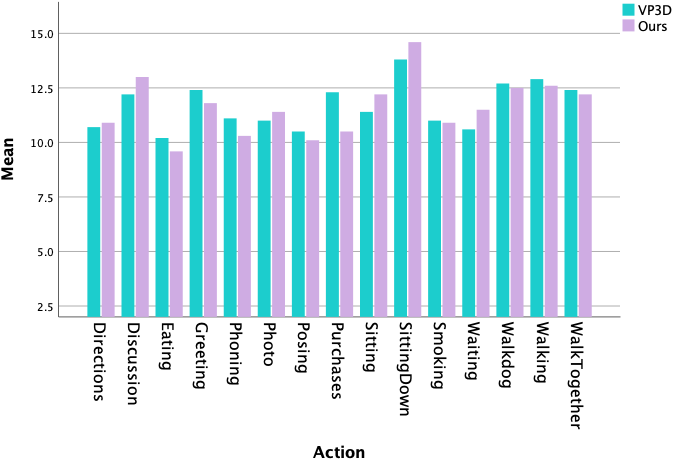
\includegraphics[width=\textwidth]{mean_error_comparison_3.png}
         \caption{1F, 15UE, Velocity Error of MPJPE}
         \label{fig:est_c}
     \end{subfigure}
     \hfill
     \begin{subfigure}[b]{0.49\textwidth}
         \centering
         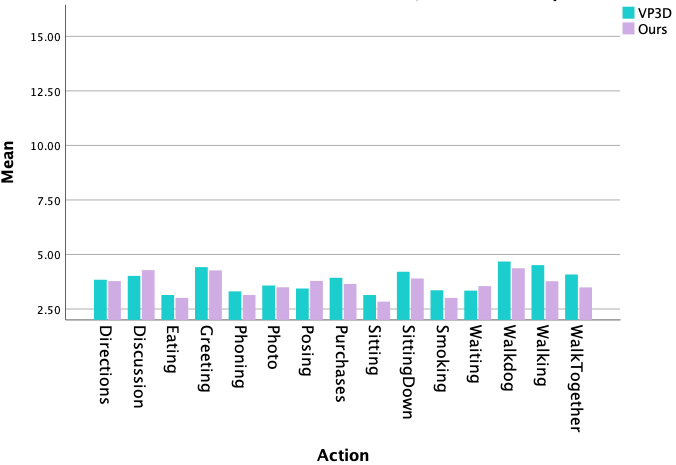
\includegraphics[width=\textwidth]{mean_error_comparison_4.png}
         \caption{\textbf{27F, 15UE, Velocity Error of MPJPE}}
         \label{fig:est_d}
     \end{subfigure}
     \hfill
        \caption{Error Visualization for experimental results}
        \label{fig:four_error_graphs}
\end{figure*}



%------------------------------------------------------------------------

\begin{table*}
\begin{minipage}[t]{.49\textwidth}
	\centering
	\begin{tabular}{ccc}
	\hline
	Object & VP3D-Avg & Ours-Avg \\
	\hline

	TC (40 E)& 84972 sec. & 28848 sec.\\
	MPJPE& 50.27 mm & 50.49 mm\\
	Velocity-M& 2.66 mm & 3.02 mm  \\
	
	\hline
	
	TC (80 E)& 176976 sec. & 56921 sec.\\
	MPJPE&  48.22 mm & 50.54 mm\\
	Velocity-M& 2.49 mm & 3.08 mm  \\
	
	\hline
	
	MPJPE $\epsilon_0$ & \multicolumn{2}{c}{60.46} \\
	Velo-M $\epsilon_0$ & \multicolumn{2}{c}{3.408} \\
	MPJPE TPR & 0.153 & 0.124 \\
	Velo-M TPR & $11.4\cdot 10^{-3}$ & $4.1\cdot 10^{-3}$ \\

	

	\hline
	\end{tabular}
\end{minipage}
\quad
\begin{minipage}[t]{.49\textwidth}
	\centering
	\begin{tabular}{ccccc}
	\hline
	Epochs & VP3D-Avg & Ours-Avg & VP3D-Eat & Ours-Eat\\
	\hline
	1 & 59.11 & 57.52 & 54.22 & 51.14 \\
	2 & 56.26 & 52.06 & 52.21 & 48.72 \\
	3 & 61.73 & 51.28 & 51.17 & 47.14 \\
	4 & 54.24 & 51.41 & 49.22 & 45.28 \\
	5 & 51.17 & 51.11 & 49.74 & 45.17\\
	6 & 50.16 & 50.11 & 51.12 & 46.28\\
	7 & 50.28 & 50.37 & 50.71 & 45.82\\
	8 & 50.19 & 50.25 & 50.23 & 47.14 \\
	9 & 50.24 & 50.34 & 49.17 & 47.22\\
	10 & 50.14 & 50.94 & 49.82 & 46.32\\
	30 & 49.56 & 50.56 & 47.71 & 45.64\\
	40 & 50.27 & 50.49 & 46.14 & 45.18\\
	50 & 48.17 & 50.29 & 45.61 & 45.12\\
	80 & 48.22 & 50.54 & 45.22 & 45.14 \\
	\hline
	\end{tabular}
\end{minipage}

\caption{The property cluster with receptive field = 243 frames and training epochs = 1200 unit epochs (left) and the 
comparison between our work and the original work under receptive field = 243 frames and training epochs = 1200 unit epochs
(right). Note that each epoch worths $15$ unit epochs.}
\label{tab:time_related}
\end{table*}

\clearpage
\newpage
\subsection{Temporal-related Training Results}

The time for training data is a crucial standard for deep learning, like the success of invention of Faster R-CNN
\cite{Ren2015}. In this part we take a deep insight of the time consumption and time-precision rate between the 
original model and our Eating-based model (left), and the relationship between our work 
and the original work using protocol MPJPE with the lapse of epochs (right) in Table \ref{tab:time_related}. The 
corresponding visualization is shown in figure \ref{fig:temporal_figure}.

In the second subtable the time-precision rate $\theta$ is calculated by the formula below, where $\epsilon_0$ stands
for the regulated error when training to the half of the process, $\epsilon_t$ represents the error 
after a long time of training (in our case 80 epochs), $i\in\{0,1\}$, $k=1.2$ and $t$ stands for the real time consumed for each training.
\begin{equation}
		\epsilon_0^{(1,2)}=\frac{\epsilon_{\left\lfloor\frac{t}{2}\right\rfloor}^{(1)}+\epsilon_{\left\lfloor\frac{t}{2}\right\rfloor}^{(2)}}{2}\cdot k
\end{equation}
\begin{equation}
	\theta^{(i)} = \frac{\epsilon_0^{(1,2)} - \epsilon_t^{(i)}}{t}
\end{equation}


\begin{figure}[H]
    \centering
    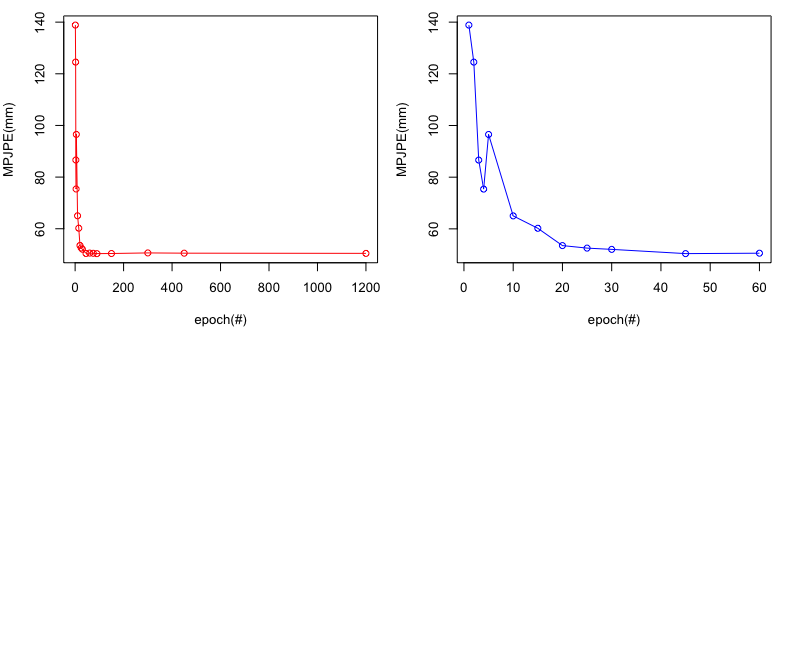
\includegraphics[width=0.49\textwidth]{MPJPE_epoch.png}
	\caption{The temporal results for the two models (\textit{VideoPose3D} and our model) and two standards (average and only eating).}
	\label{fig:temporal_figure}
\end{figure}



\section{Conclusion}

Concluding all results from the Experiment part we make conclusions that our model can be used to 

\textbf{A Solution For Action-oriented Problems.}
Our model can serve as a viable solution for action-oriented problems. For example, if there is a request that only a certain action is needed to be trained
and estimated, we can use our method to act as an alternative other than \textit{VideoPose3D}. Our model 

\subsection{Pick What You Want}

\subsection{Accelerate Training Process}

\newpage

{\small
\bibliographystyle{ieee_fullname}
\bibliography{egbib}
}

\end{document}












